% !TeX root = ../IS1_group_project.tex

\section{Value Network Analysis} \label{sec:value}

This section outlines the value flows, demonstrating how value is created and exchanged.

It models the value network within which Aethelgard Studios operates as a Value Delivery Modeling Language, see \cite{OMG_VDML},
Value Proposition Exchange Diagram.

\subsection{VDML Diagram}

The VDML Value Proposition Exchange Diagram (shown in \autoref{fig:vdml_diagram}) shows each participant as a role, and each
relationship as a pair of value propositions (VPs), one in each direction.
Every VP is an economic resource (money, goods, services or rights).

\begin{figure}[H]
    \centering
    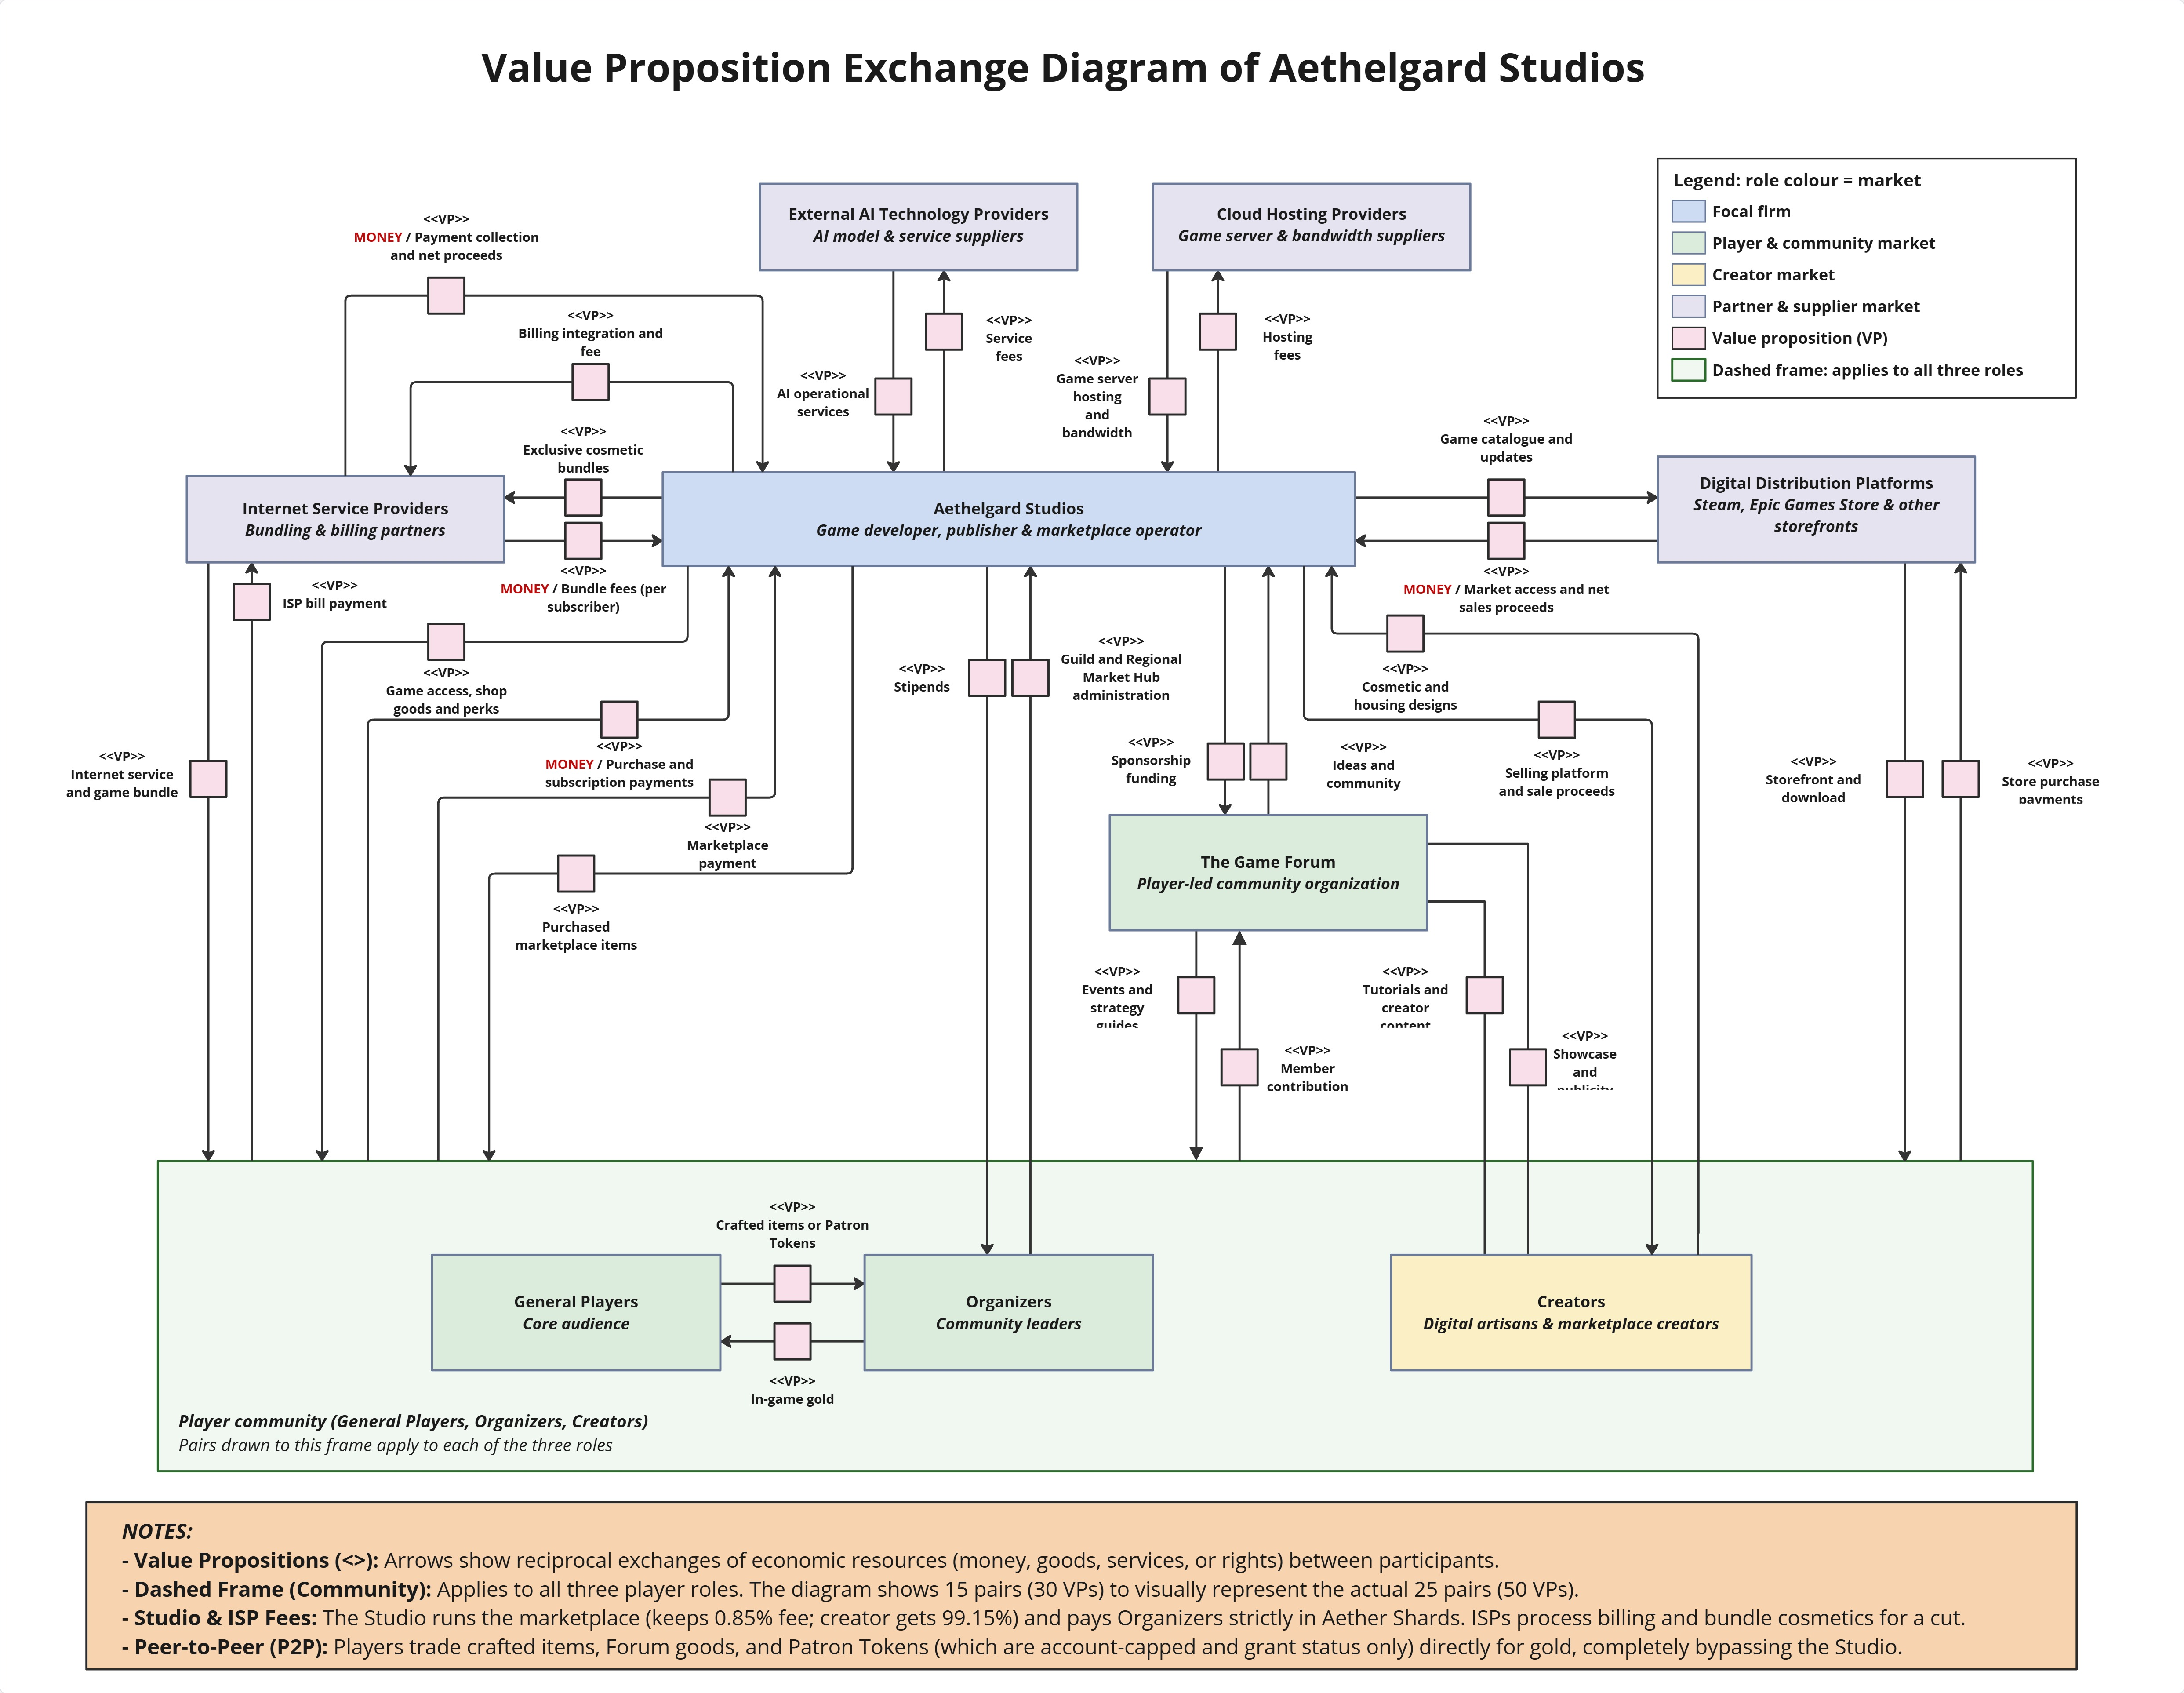
\includegraphics[width=\textwidth]{vdml_diagram}
    \caption{Value Proposition Exchange Diagram of Aethelgard Studios (VDML).}
    \label{fig:vdml_diagram}
\end{figure}

\paragraph{How to read the diagram:}
\begin{itemize}
    \item \textbf{Roles \& Markets:} Boxes represent roles, color-coded by market:
    \begin{itemize}
        \item \textcolor{blue}{\textbf{Studio}} (Blue)
        \item \textcolor{green!60!black}{\textbf{Player and Community}} (Green)
        \item \textcolor{orange}{\textbf{Creators}} (Yellow)
        \item \textcolor{purple}{\textbf{Partners and Suppliers}} (Purple)
    \end{itemize}
    \item \textbf{Value Propositions:} Pink squares represent individual Value Propositions (VPs).
    \item \textbf{Player Community Frame:} A dashed frame encompasses the player community; a relationship drawn to this frame
    applies to each of the three enclosed player roles.
\end{itemize}

\subsection{VDML Diagram Explained}

\subsubsection{Roles}

\begin{longtblr}[
    caption = {Roles participating in the value network of Aethelgard Studios.},
    label = {tab:vdml_roles}
  ]{
    colspec={X[1,l] X[1,l] X[2,l]},
    width=\textwidth,
    row{odd}={gray!15},
    row{even}={white},
    row{1}={bg=gray!90,fg=white},
    colsep=4pt
  }
    \textbf{Market} & \textbf{Role} & \textbf{Description} \\
    Focal firm & Aethelgard Studios & Develops and publishes the game, runs live services and operates the marketplace \\
    Player and community & General Players & Core audience; main buyers of cosmetics, packs and events \\
    Player and community & Organizers & Community leaders who run guilds and market hubs \\
    Player and community & The Game Forum & Player-led organisation, sponsored by the Studio, that collects improvement ideas \\
    Creator & Creators & Players who design and sell cosmetic, housing and guildhall assets \\
    Partner and supplier & Internet Service Providers & Bundle cosmetic items and collect player payments on the ISP bill \\
    Partner and supplier & Digital Distribution Platforms & Steam, Epic Games Store and other storefronts \\
    Partner and supplier & External AI Technology Providers & Models for customer service, anti-cheat and moderation \\
    Partner and supplier & Cloud Hosting Providers & Game servers, storage and bandwidth \\
\end{longtblr}

\subsubsection{Value Propositions and Deliverables}

\begin{longtblr}[
    caption = {Value propositions and their deliverables exchanged across relationships.},
    label = {tab:vdml_value_propositions}
  ]{
    colspec={Q[c, 0.6cm] X[2,l] X[3,l] X[3,l]},
    width=\textwidth,
    row{odd}={gray!15},
    row{even}={white},
    row{1}={bg=gray!90,fg=white},
    colsep=4pt
  }
    \textbf{\#} & \textbf{Relationship} & \textbf{Party 1 provides} & \textbf{Party 2 provides} \\
    1 & Studio to/from player community (play and purchases) & Game access, shop goods and perks: free game and expansions, shop goods, Patron perks & Purchase and subscription payments: payments for shop goods and Patron subscription \\
    2 & Studio to/from player community (marketplace) & Purchased marketplace items: digital delivery of the item & Marketplace payment: item price paid to the Studio \\
    3 & Studio to/from Organizers & Stipends: Aether Shard stipends (never gold), admin perks & Guild and Regional Market Hub administration: running guilds and market hubs \\
    4 & Studio to/from Creators & Selling platform and sale proceeds: tools, certification, 99.15\% of each sale & Cosmetic and housing designs: certified designs for sale (Studio keeps 0.85\%) \\
    5 & Studio to/from Game Forum & Sponsorship funding: funding, early roadmap access & Ideas and community promotion: curated player ideas, competitions, articles \\
    6 & Studio to/from Digital Distribution Platforms & Game catalogue and updates: game build and updates & Market access and net sales proceeds: reach, download service, sales proceeds net of commission \\
    7 & Studio to/from ISPs (bundling) & Exclusive cosmetic bundles: bundles for the ISP's subscribers & Bundle fees (per subscriber): fee per activated subscriber \\
    8 & Studio to/from ISPs (billing) & Billing integration and fee: payment integration with the ISP bill; ISP keeps a billing fee & Payment collection and net proceeds: player payments collected, passed on net of the fee \\
    9 & Studio to/from AI providers & Service fees: fees for contracted AI & AI operational services: hosted models under agreed service levels \\
    10 & Studio to/from Cloud hosting & Hosting fees: monthly pay-as-you-go fees & Game server hosting and bandwidth: servers, storage, delivery under agreed uptime \\
    11 & ISPs to/from player community & Internet service and game bundle: connectivity including the bundle & ISP bill payment: subscription and Studio purchases paid on the bill \\
    12 & Platforms to/from player community & Storefront and download service: discovery, download, patching & Store purchase payments: in-game purchases made through the store \\
    13 & Game Forum to/from player community & Events and strategy guides: community events and guides & Member contribution: articles, rankings, volunteer effort \\
    14 & Game Forum to/from Creators & Showcase and publicity: showcase of creators' work & Tutorials and creator content: tutorials and creator-made content \\
    15 & General Players to/from Organizers & Crafted items or Patron Tokens: items and tokens offered on the auction house & In-game gold: gold paid by the buyer \\
\end{longtblr}

\subsubsection{Key Points}

\begin{itemize}
    \item \textbf{Marketplace:} Buyers pay the Studio, the Studio delivers the item and pays the creator 99.15\%, keeping 0.85\%.
    Every payment passes through the Studio.
    \item \textbf{ISPs:} Two separate pairs. In bundling, the ISP pays a fee per activated subscriber.
    In billing, the ISP collects player payments and keeps a fee before passing the rest on.
    \item \textbf{Player trade (row 15):} A role cannot exchange with itself, so this pair stands for all player-to-player trade.
    Either role can sell or buy, and the Studio is not involved.
    \item \textbf{Fairness:} Stipends are paid in Aether Shards, never gold, and Patron Tokens grant status only, with sales
    capped per account (\autoref{sec:value}).
    \item \textbf{Why the Studio gives value:} Payments, fees and net proceeds are revenue. AI and hosting keep the game running.
    Creator designs, Organizer administration and Forum ideas bring content, community management and feedback that support
    retention.
\end{itemize}

\subsubsection{Assumptions}

\begin{enumerate}
    \item The case's two segments are modelled as three roles: General Players, Organizers and Creators. Creators also buy and
    play, so shared pairs apply to all three.
    \item Steam, Epic and similar storefronts are one role, because the value exchanged is the same.
    \item The ISP has two relationships with the Studio (bundling and billing). Fee amounts are not modelled.
    \item AI and hosting are bought from external vendors.
    \item Crafted items and in-game gold are virtual goods and a virtual currency that can be priced, so their trade is modelled.
    \item Only the 0.85\% fee is given by the case. Other prices are left out, since a value network records the type of
    deliverable, not its price.
    \item Payment processing for the Studio's own launcher is part of the Studio, and investors are outside the network.
\end{enumerate}
